\documentclass[12pt,twoside]{article}
\usepackage{light}
\usepackage{subfigure}
\usepackage{enumitem}
\usepackage{graphicx}
\hidesolutions
%\showsolutions

%Solutions are currently incorrect
\begin{document}

\begin{problem}{15}
Refer to the following graph for parts a, b:
\begin{figure}[!ht]
\begin{center}
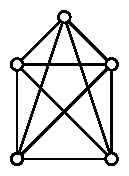
\includegraphics[width=3cm]{GridGraph.pdf}\end{center}
\end{figure}


\bparts
\ppart{3} Does the above graph have a Hamiltonian path?
\solution{
Yes.  We can start at a single vertex and just traverse the cycle formed by the outer edges to form the Hamiltonian path.
}
\ppart{3} Does the above graph have a Eulerian path?
\solution{
Yes.  Each vertex has even degree so in fact this graph has an Eulerian cycle.
}

\ppart{9} Consider the complete graph on $n$ vertices $K_n$ for odd $n \geq 3$.  Prove that we cannot find a series of Hamiltonian paths in $K_n$ that together cover all the edges of $K_n$.  

\solution{
Each Hamiltonian path contains $n-1$ edges.  There are $\frac{n(n-1)}{2}$ edges in the complete graph.  Hence if we were to be able to decompose $K_n$ into Hamiltonian paths, we must have $ n-1 \mid \frac{n(n-1)}{2}$ and so $2 \mid n$.  This is never true if $n$ is odd.  
}

\eparts
\end{problem}

%%%%%%%%%%%%%%%%%%%%%%%%%%%%%%%%%%%%%%%%%%%%%%%%%%%%%

\newpage

%%%%%%%%%%%%%%%%%%%%%%%%%%%%%%%%%%%%%%%%%%%%%%%%%%%%%


\begin{problem}{15}
\bparts
\ppart{3} Find $7^{100}$ mod $13$.
\solution{
We use Fermat's little theorem to first note that $7^12 \equiv 1$ (mod $13$).  Hence $7^{96} \equiv 1$ (mod $13$).  Hence we have that $7^{100} \equiv 7^4$ (mod $13$).  We know $49 \equiv -3$ (mod $13$) and so $7^4 \equiv -3 \cdot -3 = 9$ (mod $13$).  Hence $7^{100} \equiv 9$ (mod $13$).  
}
\ppart{3} Find the inverse of $33$ mod $121$ or prove that no such inverse exists.
\solution{
There is no inverse for $33$ mod $121$.  Suppose that $x$ is the inverse of $33$ mod $121$.  Then we have that $33x - 1 = 121y$ for some integer $y$.  This means that $11 \mid 1$, which is a contradiction.  
}
\ppart{4} Prove that for any non-zero integers $a, b, c, d$, if $a - c \mid ab + cd$, then $a - c \mid ad + bc$.
\solution{
We have that $a - c \mid ab + cd$.  This implies $a - c \mid ab - cb + cb - ad + ad + cd = (a-c)b + (c-a)d + ad + bc$.  Now $a-c \mid a-c$ and $a-c \mid c-a$, and so we have that $a-c$ must divide $ad + bc$.  
}

\ppart{5} Show that any perfect square is of the form $3k$ or $3k + 1$ but never of the form $3k + 2$ for integer $k$.  

\solution{
Suppose we have some integer $x$.  Then $x$ can leave a remainder 0, 1, 2 when considered mod 3.  This would imply $x^2$ leaves a remainder 0, 1, 1 when considered mod 3.  This means that $x^2$ only leaves a remainder $0$ or $1$ mod 4 and so $x^2$ is either of the form $3k$ or $3k+1$ but never of the form $3k+2$ as desired.  
}
\eparts
\end{problem}

%%%%%%%%%%%%%%%%%%%%%%%%%%%%%%%%%%%%%%%%%%%%%%%%%%%%%

\newpage

%%%%%%%%%%%%%%%%%%%%%%%%%%%%%%%%%%%%%%%%%%%%%%%%%%%%%


\begin{problem}{10}
Suppose we are planning a trip to California for Thanksgiving.  Unfortunately, we are booking our tickets late and so the prices are all really high. Suppose we are given the following list of ticket prices and travel times:

\begin{enumerate}[label=\Alph*]
\item 600 dollars, 9 hours 20 minutes
\item 650 dollars, 8 hours 40 minutes
\item 550 dollars, 9 hours 10 minutes
\item 575 dollars, 8 hours 20 minutes
\item 660 dollars, 9 hours 5 minutes
\end{enumerate}

Our goal is to find the tickets that are the cheapest while minimizing travel time.

\bparts
\ppart{4} Suppose we had the ordering $\leq$ such that for tickets $i, j$ $i \leq j$ if $i$ is at least as expensive as $j$ and $i$'s travel time is at least as long as $j$'s travel time.  

\solution{
We show that the relation is reflexive:  This is clear, as each ticket is at least as expensive as itself and the travel time per ticket is equal to itself.

We show that the relation is anti-symmetric: Suppose tickets $i,j$ satisfy $i \leq j$ and $j \leq i$. Then ticket $i$ is at least as expensive as ticket $j$ and ticket $j$ is at least as expensive as ticket $j$ so their prices must be equal.  Similarly, ticket $i$'s travel time is at least as long as ticket $j$'s travel time and so ticket $i$ and $j$ have the same travel time.  Hence they are the same ticket.

We show that the relation is transitive: Suppose we have tickets $i, j, k$ such that $i \leq j$ and $j \leq k$.  Then $i$ is at least as expensive as $j$ and $j$ is at least as expensive as $k$, so $i$ is at least as expensive as $k$.  Similarly, $i$'s travel time is at least as long as $j$'s travel time and $j$'s travel time is at least as long as $k$'s travel time.  Hence $i$'s travel time is at least as long as $k$'s travel time.
}

\ppart{3} Draw the Hasse diagram for the above tickets with the ticket $i$ is $<$ ticket $j$ if ticket $i$ is both more expensive and has more travel time than ticket $j$.

\ppart{3} Find the maximal elements of the poset.  Is there a maximum element? 

\solution{
Tickets $C$ and $D$ are maximal elements in this poset.  There is no maximum element for this poset.
}
\eparts
\end{problem}

%%%%%%%%%%%%%%%%%%%%%%%%%%%%%%%%%%%%%%%%%%%%%%%%%%%%%

\newpage

%%%%%%%%%%%%%%%%%%%%%%%%%%%%%%%%%%%%%%%%%%%%%%%%%%%%%


\begin{problem}{10} 
A portion of a computer program consists of a sequence of calculations
where the results are stored in variables, like this:
\[
\begin{array}{rrrcl}
&& \text{Inputs:} &  & x, y \\
\text{Step } 1. & \hspace{0.5in} & a & = & x - 24 \\
2. && b & = & x * a \\
3. && c & = & 3 \\
4. && d & = & y - c \\
5. && e & = & y ** c \\
6. && f & = & e + 1  \\
&& \text{Outputs:} & & b, d, e
\end{array}
\]
A computer can perform such calculations most quickly if the value of
each variable is stored in a \emph{register}, a chunk of very fast
memory inside the microprocessor.  Programming language compilers face
the problem of assigning each variable in a program to a register.
Computers usually have few registers, however, so they must be used
wisely and reused often.  This is called the \emph{register
  allocation} problem.

In the example above, variables $x$ and $y$ must be assigned different
registers, because they hold distinct input values.  Furthermore, $c$
and $d$ must be assigned different registers; if they used the same
one, then the value of $c$ would be overwritten in the fourth step and
we'd get the wrong answer in the fifth step.  On the other hand,
variables $b$ and $d$ may use the same register; we no longer need $b$ and can overwrite the register that holds its
value.  Assume that the computer carries out each step in the order
listed and that each step is completed before the next is begun.

\bparts

\ppart{7} Recast the register allocation problem as a question
about graph coloring.  What do the vertices correspond to?  Construct
the graph corresponding to the example above.

\solution{
There is one vertex for each variable.  An edge between two vertices
indicates that the values of the variables must be stored in different
registers.  We can tell when two variables must be stored in different
registers as follows: classify each appearance of a variable in the
program as either an \emph{assignment} or a \emph{use}.  An appearance
is an \emph{assignment} when the variable is on the left side of an
equation or on the ``Inputs'' line.  An appearance of a variable is a
\emph{use} if the variable is on the right side of
an equation or on the ``Outputs'' line.  The \emph{lifetime} of a variable is the segment of code
extending from the initial assignment of the variable until the last
use.  There is an edge between two variables iff their lifetimes
overlap.

  We are also assuming that all variables are relevant to the Outputs,
  where a variable is \emph{relevant} iff it
  is an Output or is used in an assignment to a relevant variable.
  This is a recursive---not a circular---definition of relevant
  variable!

  Likewise, we assume that all variables are \emph{dependent} on the Inputs, where a variable is
  dependent on the Inputs iff it is an Input or appears in the left
  hand side of an assignment whose right hand side contains a
  dependent variable.
}

\ppart{3} How many registers
do you need?

\solution{
Four registers are needed.

One possible assignment of variables to registers is indicated in the
figure above.  In general, coloring a graph using the minimum number
of colors is quite difficult; no efficient procedure is known.
However, the register allocation problem always leads to an
\term{interval graph}, and optimal colorings for interval graphs are
always easy to find.  This makes it easy for compilers to allocate a
minimum number of registers.
}


%%%%%%%%%%%%%%%%%%%%%%%%%%%%%%%%%%%%%%%%%%%%%%%%%%%%%

\newpage

%%%%%%%%%%%%%%%%%%%%%%%%%%%%%%%%%%%%%%%%%%%%%%%%%%%%%


\begin{problem}{15} 
Use the web graph below to answer parts (a), (b), and (c) of this question. The pagerank of vertex $i$ can be written as $p_i$. 

\begin{figure}[!ht]
\begin{center}
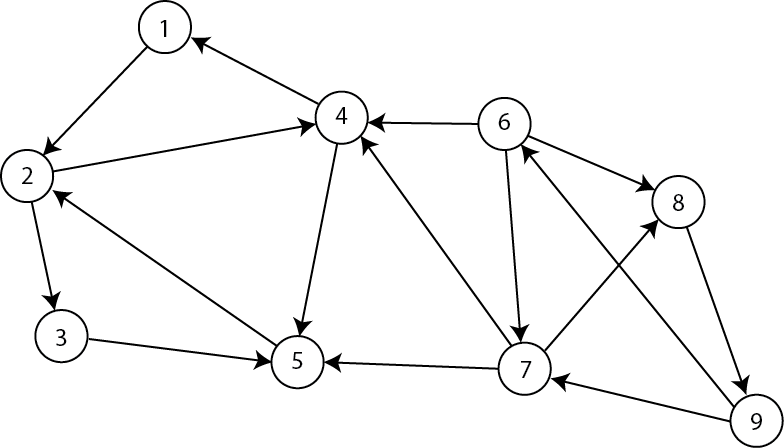
\includegraphics[width=12cm]{pagerank.png}\end{center}
\caption{Web Graph}
\end{figure}

\bparts

\ppart{5} For $\vec{p}~'$ in terms of $\vec{p}$ can be written as a matrix product: $\vec{p}~' = W\vec{p}$, for some matrix $W$, which is the \emph{update matrix}. Find the update matrix.

\solution{
\[
\begin{bmatrix}
    0 & 0 & 0 & \frac{1}{2} & 0 & 0 & 0 & 0 & 0 \\
    1 & 0 & 0 & 0               & 1 & 0 & 0 & 0 & 0 \\
    0 & \frac{1}{2} & 0 & 0 & 0 & 0 & 0 & 0 & 0 \\
    0 & \frac{1}{2} & 0 & 0 & 0 & \frac{1}{3} & \frac{1}{3} & 0 & 0 \\
    0 & 0 & 1 & \frac{1}{2} & 0 & 0 & \frac{1}{3} & 0 & 0 \\
    0 & 0 & 0 & 0 & 0 & 0 & 0 & 0 & \frac{1}{2} \\
    0 & 0 & 0 & 0 & 0 & \frac{1}{3} & 0 & 0 & \frac{1}{2} \\
    0 & 0 & 0 & 0 & 0 & \frac{1}{3} & \frac{1}{3} & 0 & 0 \\
    0 & 0 & 0 & 0 & 0 & 0 & 0 & 1 & 0 \\
    
\end{bmatrix}
\]
}

\ppart{3} Which (if any) of the vertices of the web graph above will have PageRank value tending to zero if we run the PageRunk algorithm for many (let's say 200,000) iterations?

\solution{
The vertices 6, 7, 8, 9 will have PageRank value tending to 0.  This is because 6, 7, 8, 9 form a strongly connected component with edges only going toward a second strongly component formed by 1, 2, 3, 4, 5.  The result then follows from the result of problem 4b on the last homework.  
}

\ppart{7} Suppose we remove all the vertices that you found in part b from our Web Graph along with all corresponding edges from those vertices and consider the remaining graph $G$.  Find the normalized stationary distribution across the nodes assuming that each node in $G$ starts with uniform values.
  
\textbf{Note}: If you are not confident about your answer in part b, feel free to instead find the stationary distribution for the directed triangle formed by vertices 1, 2, 4 of the Web Graph.  Again assume each of the nodes 1, 2, 4 starts with inital PageRank value $\frac{1}{3}$.  

\solution{
We consider the distribution across vertices 1, 2, 3, 4, 5 as these will have non-zero PageRank values in the long run.  Considering only the upper 5 x 5 entries in the PageRank matrix from part a, we have the following system of equations:

\begin{equation}
\begin{split}
v_1 &= \frac{1}{2}v_2 \\
v_2 &= v_1 + v_5 \\
v_3 &= \frac{1}{2}v_2 \\
v_4 &= \frac{1}{2}v_2 \\
v_5 &= v_3 + \frac{1}{2}v_4 \\
v_1 + v_2 + v_3 + v_4 + v_5 &= 1 \\
\end{split}
\end{equation}
Solving the system of equations, we find that the solution is $v_1 = \frac{1}{12}, v_2 = \frac{1}{3}, v_3 = \frac{1}{6}, v_4 = \frac{1}{6}, v_5 = \frac{1}{4}$.


If the student chose instead to solve the problem listed in the note, then the solution is just $\frac{1}{3}$ for each vertex 1, 2, 4.  

}


\eparts
\end{problem}

\eparts
\end{problem}


%%%%%%%%%%%%%%%%%%%%%%%%%%%%%%%%%%%%%%%%%%%%%%%%%%%%%

\newpage

%%%%%%%%%%%%%%%%%%%%%%%%%%%%%%%%%%%%%%%%%%%%%%%%%%%%%

\begin{problem}{10}
A \emph{multiple binary-tree network} has $n$ inputs and $n$ outputs, where $n$ is
a power of 2.  Each input is connected to the root of a binary tree with
$n/2$ leaves and with edges pointing away from the root.  Likewise, each
output is connected to the root of a binary tree with $n/2$ leaves and
with edges pointing toward the root.

Two edges point from each leaf of an input tree, and each of these edges
points to a leaf of an output tree.  The matching of leaf edges is
arranged so that for every input and output tree, there is an edge from a
leaf of the input tree to a leaf of the output tree, and every output tree
leaf has exactly two edges pointing to it.

\bparts
\ppart{4} Draw such a multiple binary-tree net for $n=4$.

\solution{
\begin{figure}[h]
%\graphic{binnet}
\centering
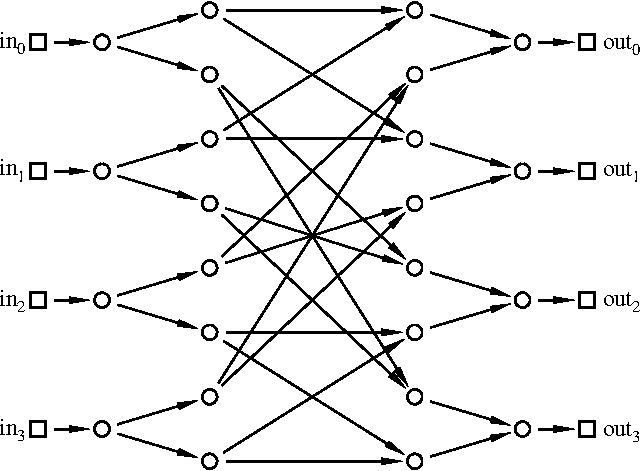
\includegraphics[scale=1]{binnet}
\end{figure}
}

\ppart{6} Fill in the table, and explain your entries.

{\large
\[
\begin{array}{c|c|c|c}
\text{\# switches} &
\text{switch size} &
\text{diameter} &
\text{max congestion} \\ \hline
&&&\\ \hline
\end{array}
\]
}


\solution{
{\large
\[
\begin{array}{c|c|c|c}
\text{\# switches} &
\text{switch size} &
\text{diameter} &
\text{max congestion} \\ \hline
2n(n-1)& 1 \times 2, 2 \times 1 & 1+ 2\log n & 1\\ \hline
\end{array}
\]
}

\iffalse
\begin{align*}
\text{\# switches } & = 2n(n-1)\\
\text{switch size} & = 1 \times 2, 2 \times 1\\
\text{diameter} & =  1+ 2\log n\\
\text{max congestion} & =1
\end{align*}
\fi

These formulas were gotten as follows: a binary tree with $n/2$ leaves has
$n-1$ nodes (switches), and there are $2n$ trees.

Each node of an input tree has one edge in and two out; the opposite
for nodes of output trees.

The distance from any input to any output is 1 from input to tree root,
$(\log n)-1$ from root to leaf, 1 from input leaf to output leaf, $(\log
n)-1$ from output leaf to output root, and 1 to output, for a total of $1+
2\log n$.

The path from any input to any output is unique, and paths from two inputs
to different outputs don't overlap, so at most one packet goes through any
switch.
}

\eparts

\end{problem}

%%%%%%%%%%%%%%%%%%%%%%%%%%%%%%%%%%%%%%%%%%%%%%%%%%%%%

\newpage

%%%%%%%%%%%%%%%%%%%%%%%%%%%%%%%%%%%%%%%%%%%%%%%%%%%%%


\begin{problem}{10}
There are $n \geq 1$ identical cars on a circular track for some integer $n$. Among all of them, they have just enough gas for one car to complete a lap. Show that there is a car which can complete a lap by collecting gas from the other cars on its way around. (Hint: use induction)

\solution{
We prove this by using induction.

Base case: For $n = 1$, we are given that the car has enough gas to go around the track.

Inductive Hypothesis: Suppose for $n = k$, there is one among the $k$ cars that can collect gas from the other cars on its way around and complete the lap.  

Inductive Step: Suppose $n = k + 1$.  We first find a car $A$ that has enough gas to get to the next car $B$.  This must be true since if there was no such car, then no car could ever get to the next car and so the cars together would not have enough gas to get around the track.  Let us then empty all of the gas from car $B$ into car $A$ and remove car $B$ from the track.  Then, we now have $k$ cars with enough gas to go around the track.  Now placing back car $B$, we must have that whatever car among the $k$ cars that had enough gas to get around to car $A$ can get to car $B$ because car $A$ had enough gas to get to car $B$.  Hence there is some car can get around the entire track. 

As the statement is true for $n = k+1$, we can conclude that the statement holds for all positive integers.

}

\end{problem}

%%%%%%%%%%%%%%%%%%%%%%%%%%%%%%%%%%%%%%%%%%%%%%%%%%%%%

\newpage

%%%%%%%%%%%%%%%%%%%%%%%%%%%%%%%%%%%%%%%%%%%%%%%%%%%%%


\begin{problem}{15}
Use the matrix below and the invariance principle to prove the following statements. 
\[
\begin{bmatrix}
    1 & 1 & 1 & 1 \\
    1 & 1 & 1 & 1 \\
    1 & 1 & 1 & 1 \\
    1 & -1 & 1 & 1 \\
\end{bmatrix}
\]

\bparts
\ppart{5} Suppose we are allowed to flip all of the signs of entries in any row or column.  Prove that at least one -1 will remain in the matrix.

\solution{
Consider the product of all the elements in this matrix.  We claim that this is invariant under any of the operations provided.  Suppose we flip all the signs of an element in one row.  Then if there were previously $b$ -1's in that row, then there are now $4-b$ -1's in that row and $b$ 1's in that row.  However, $4-b$ and $b$ have the same parity for integer $b = 0, 1, 2, 3, 4$.  Hence, the product remains invariant under a row operation.  A similar argument can be used for the column operation.  Hence as the product is initially -1, the product will always be -1 after any number of row or column operations and so there will always be at least one -1 in the matrix.
}

\ppart{10} Suppose that we are allowed to flip all of the signs of entries in any row, column, or a parallel to one of the diagonals.  In particular, you may switch the sign of each corner square.  Prove that at least one -1 will remain in the matrix.  

\solution{This is tricky.  Our invariant will be the product of elements on the 8 non-corner boundary entries of our matrix.  Under any of the row or column operations only two elements of these 8 are flipped and the product remains the same.  Similarly for any operation along a parallel to the diagonal flips either two or 0 or these elements.  Hence the product is again invariant.  Now as the initial product of these entries is -1 and the product is invariant, there must always be at least one -1 in the matrix.    

}
\eparts

\end{problem}


\end{document}
